% ****** Start of file bhextractor_paper.tex ******
%

\documentclass[%
 reprint,
%superscriptaddress,
%groupedaddress,
%unsortedaddress,
%runinaddress,
%frontmatterverbose, 
%preprint,
%showpacs,preprintnumbers,
%nofootinbib,
%nobibnotes,
%bibnotes,
 amsmath,amssymb,
 aps,
%pra,
%prb,
%rmp,
%prstab,
%prstper,
%floatfix,
]{revtex4-1}

\usepackage{graphicx}% Include figure files
\usepackage{dcolumn}% Align table columns on decimal point
\usepackage{bm}% bold math
%\usepackage{hyperref}% add hypertext capabilities
%\usepackage[mathlines]{lineno}% Enable numbering of text and display math
%\linenumbers\relax % Commence numbering lines

%\usepackage[showframe,%Uncomment any one of the following lines to test 
%%scale=0.7, marginratio={1:1, 2:3}, ignoreall,% default settings
%%text={7in,10in},centering,
%%margin=1.5in,
%%total={6.5in,8.75in}, top=1.2in, left=0.9in, includefoot,
%%height=10in,a5paper,hmargin={3cm,0.8in},
%]{geometry}

\begin{document}

\preprint{APS/123-QED}

\title{Black Hole Evidence Extractor}% Force line breaks with \\
%\thanks{This paper is awesome. You are awesome}%

\author{Alexander Lombardi}
 \affiliation{Physics Department, University of Massachusetts.}
 \email{alombardi@physics.umass.edu}
\author{James Clark}
 \affiliation{Physics Department, Georgia Institute of Technology.}%
 \email{james.clark@physics.gatech.edu}
\author{Laura Cadonati}
 \affiliation{Physics Department, Georgia Institute of Technology.}%
 \email{laura.cadonati@physics.gatech.edu}
\collaboration{LIGO Scientific Collaboration (LSC)}

\date{\today}

\begin{abstract}
% Verbatim from Sant Cugat Paper
Despite recent progress in numerical simulations of the coalescence of binary black hole systems, the simulation of highly asymmetric spinning systems and the construction of accurate physical templates remain challenging and computationally expensive. We explore the feasibility of a prompt and robust test of whether the signals exhibit evidence for generic features that can educate new simulations. We form catalogs of numerical relativity waveforms with distinct physical effects and compute the relative probability that a gravitational wave signal belongs to each catalog. We introduce an algorithm designed to perform this task for coalescence signals using principal component analysis of waveform catalogs and Bayesian model selection and demonstrate its effectiveness.
\end{abstract}

%\pacs{Valid PACS appear here}% PACS, the Physics and Astronomy
                             % Classification Scheme.
%\keywords{Suggested keywords}%Use showkeys class option if keyword
                              %display desired
\maketitle

%\tableofcontents

\section{Introduction}
% Verbatim from Sant Cugat Paper
The coalescence of two black holes is arguably the most powerful source of gravitational waves (GWs) detectable by the second generation of ground based detectors: Advanced LIGO (Harry, 2010), Advanced Virgo (Acernese et al., 2009), and KAGRA (Somiya, 2012). The discovery of these signatures, forecast within the next few years (Aasi et al., 2013b), will open a new era of gravitational wave astrophysics, where the GW signature will provide insights on the physical properties of the source. To decode the information in the GW waveform, we need a careful mapping with the masses and the spin magnitude and orientation of the black holes; this is the charge of numerical relativity (NR).

While available NR waveforms span an increasing portion of the physical parameter space of unequal mass, spin and precession binary black holes (BBHs) (Ajith et al., 2012; Hinder et al., 2014), each simulation takes a week or more to run. A complete coverage of the full parameter space remains a slow but important endeavor to enable GW matched filtering and parameter estimation (Thorne, 1987; Aasi et al., 2013a). The LIGO and Virgo Collaborations have refined techniques for the search of generic gravitational wave transients, or bursts, which don't assume a specific waveform but rely on a coherent GW in multiple detectors for a variety of plausible sources (Abadie et al., 2012; Andersson et al., 2013). The work presented here aims to answer the question of how a transient detected by a template-less burst search can trigger new NR simulations in interesting regions of the BBH parameter space. We introduce a proof-of-concept study, which uses the method of Principal Component Analysis (PCA) to compare a plausible signal to catalogs of NR waveforms, which represent certain regions of the BBH physical parameter space.

\section{Binary Black Hole Merger Simulations}
% Verbatim from Sant Cugat Paper
The GW waveform produced by solar and intermediate mass BBH systems spans the sensitive band of ground based detectors through the inspiral, merger and ring- down phases. While post-Newtonian and perturbation theories adequately describe the inspiral and ringdown, numerical relativity is necessary to capture the physics of the merger. NR has been successfully moving through the parameter space of binary black hole mergers since the breakthrough of 2005 (Pretorius, 2005) achieving extreme mass ratios (Lousto and Zlochower, 2011), extreme spin magnitudes (Lovelace et al., 2012) and many precessing runs (Mroue et al., 2013; Pekowsky et al., 2013).

The NR waveforms used in this paper were produced by the MAYA code of the Georgia Institute of Technology (Vaishnav et al., 2007) The MAYA code uses the Einstein Toolkit, which is based on the CACTUS infrastructure and CARPET mesh refinement (Schnetter et al., 2004). The output of all simulations is the Weyl Scalar, $\psi_4$, decomposed into spin-weighted spherical harmonics that is then converted to strain (Reisswig and Pollney, 2011).

For this work we use 48 NR runs, listed in Table 1 without hybridization with post-Newtonian waveforms. The Q-series contains 13 non-spinning, unequal-mass simulations. We use 15 runs from the HR-series, a set of unequal-mass, equal spin simulations, with initial spin parallel to the initial angular momentum. The RO3-series is a set of 20 unequal-mass simulations with the lighter black hole spin aligned to the initial angular momentum (z-axis) and the other black hole at a tilt angle $\theta$ with the z-axis in the xz-plane; these systems are precessing and the tilt-angles are defined at a specific separation of the black holes at one instant in the evolution of the binary system and change in time. While the runs are tabulated with initial parameters, there is no functional form to relate one waveform to the next; we use a Principal Component Analysis to determine the differences in each catalog and how to best capture their signatures on the data.

\section{Waveform Catalogs}

\begin{figure}
\centering
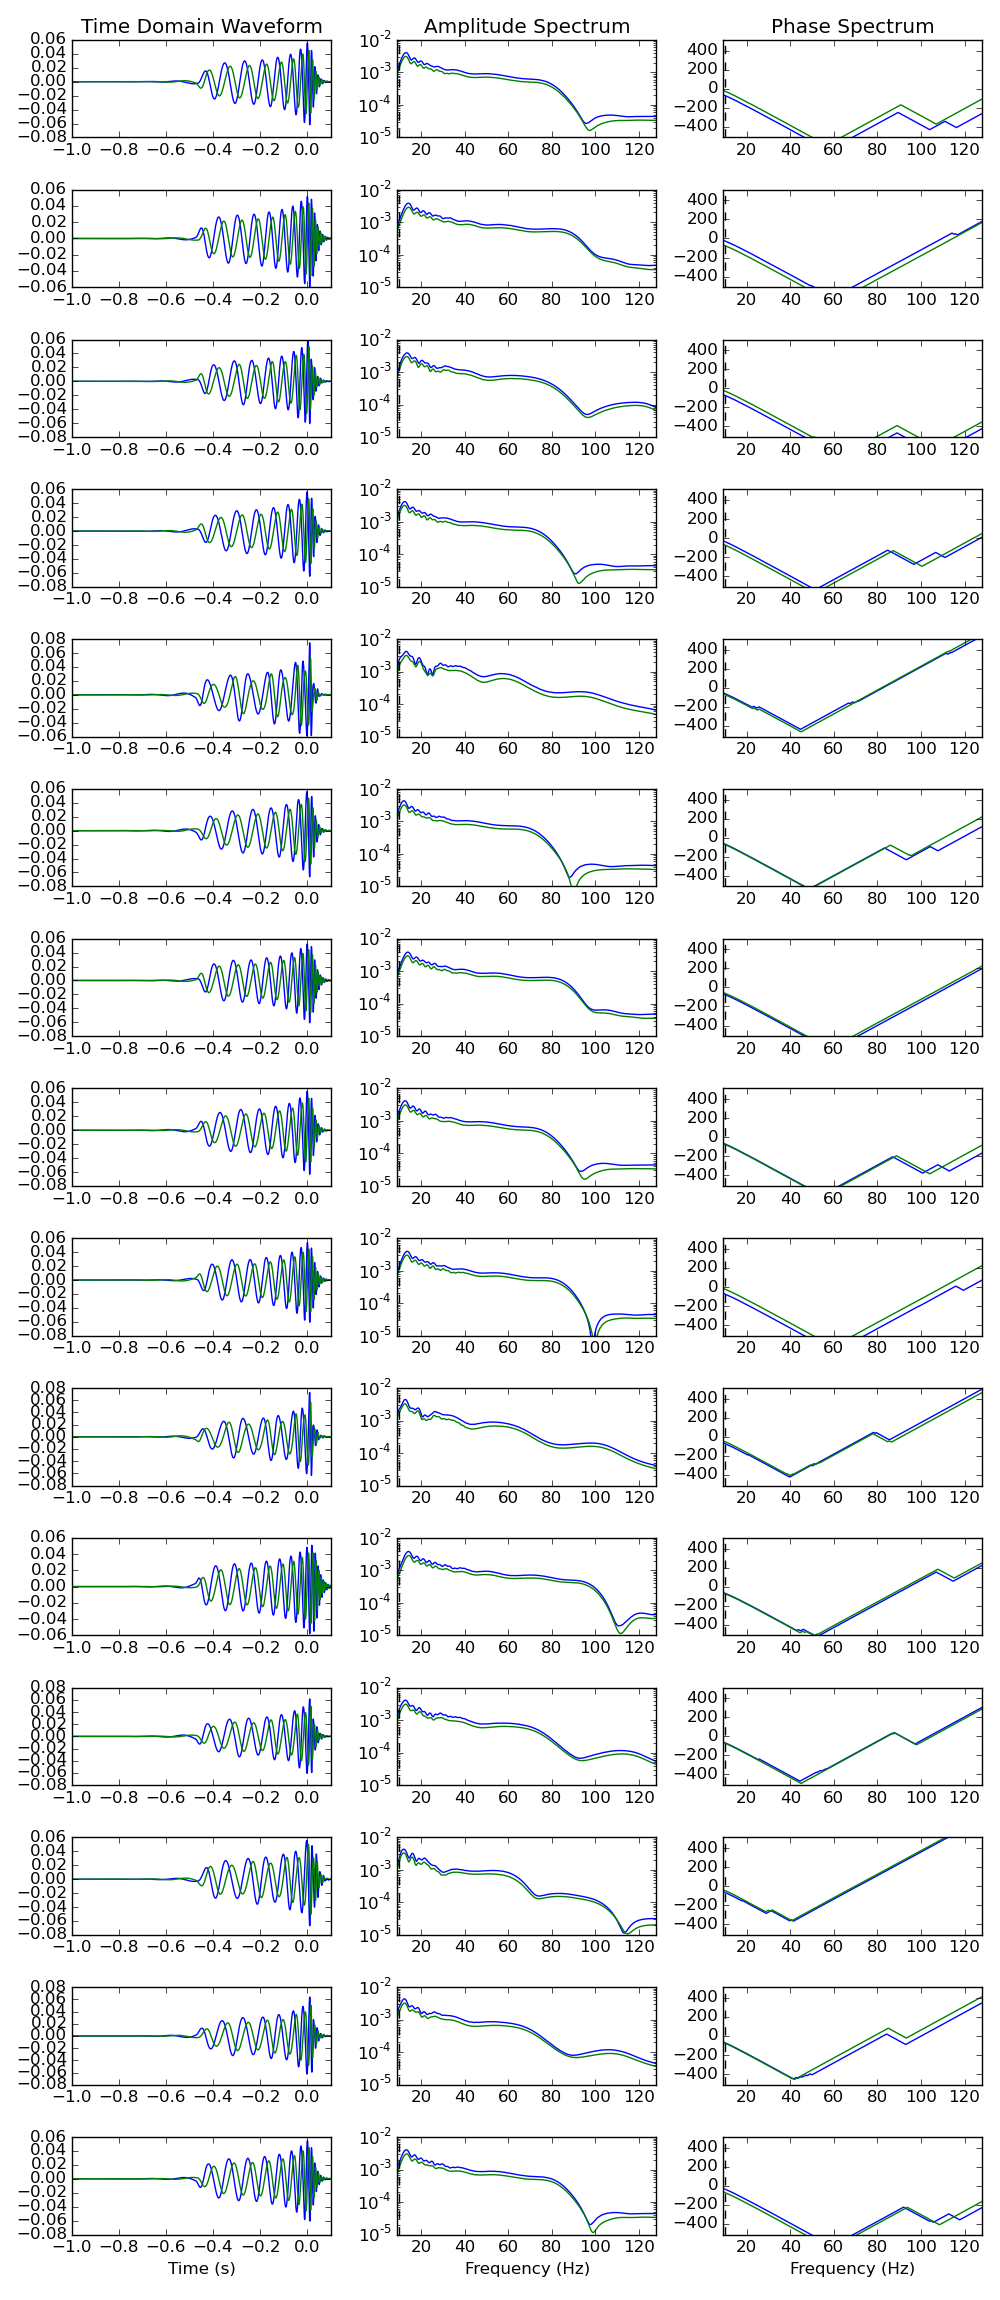
\includegraphics[width=0.4\textwidth]{figures/HR-series_catalogue.png}
\caption{Waveforms that make up the HR catalog}
\label{fig:HR_catalog}
\end{figure}

\begin{figure}
\centering
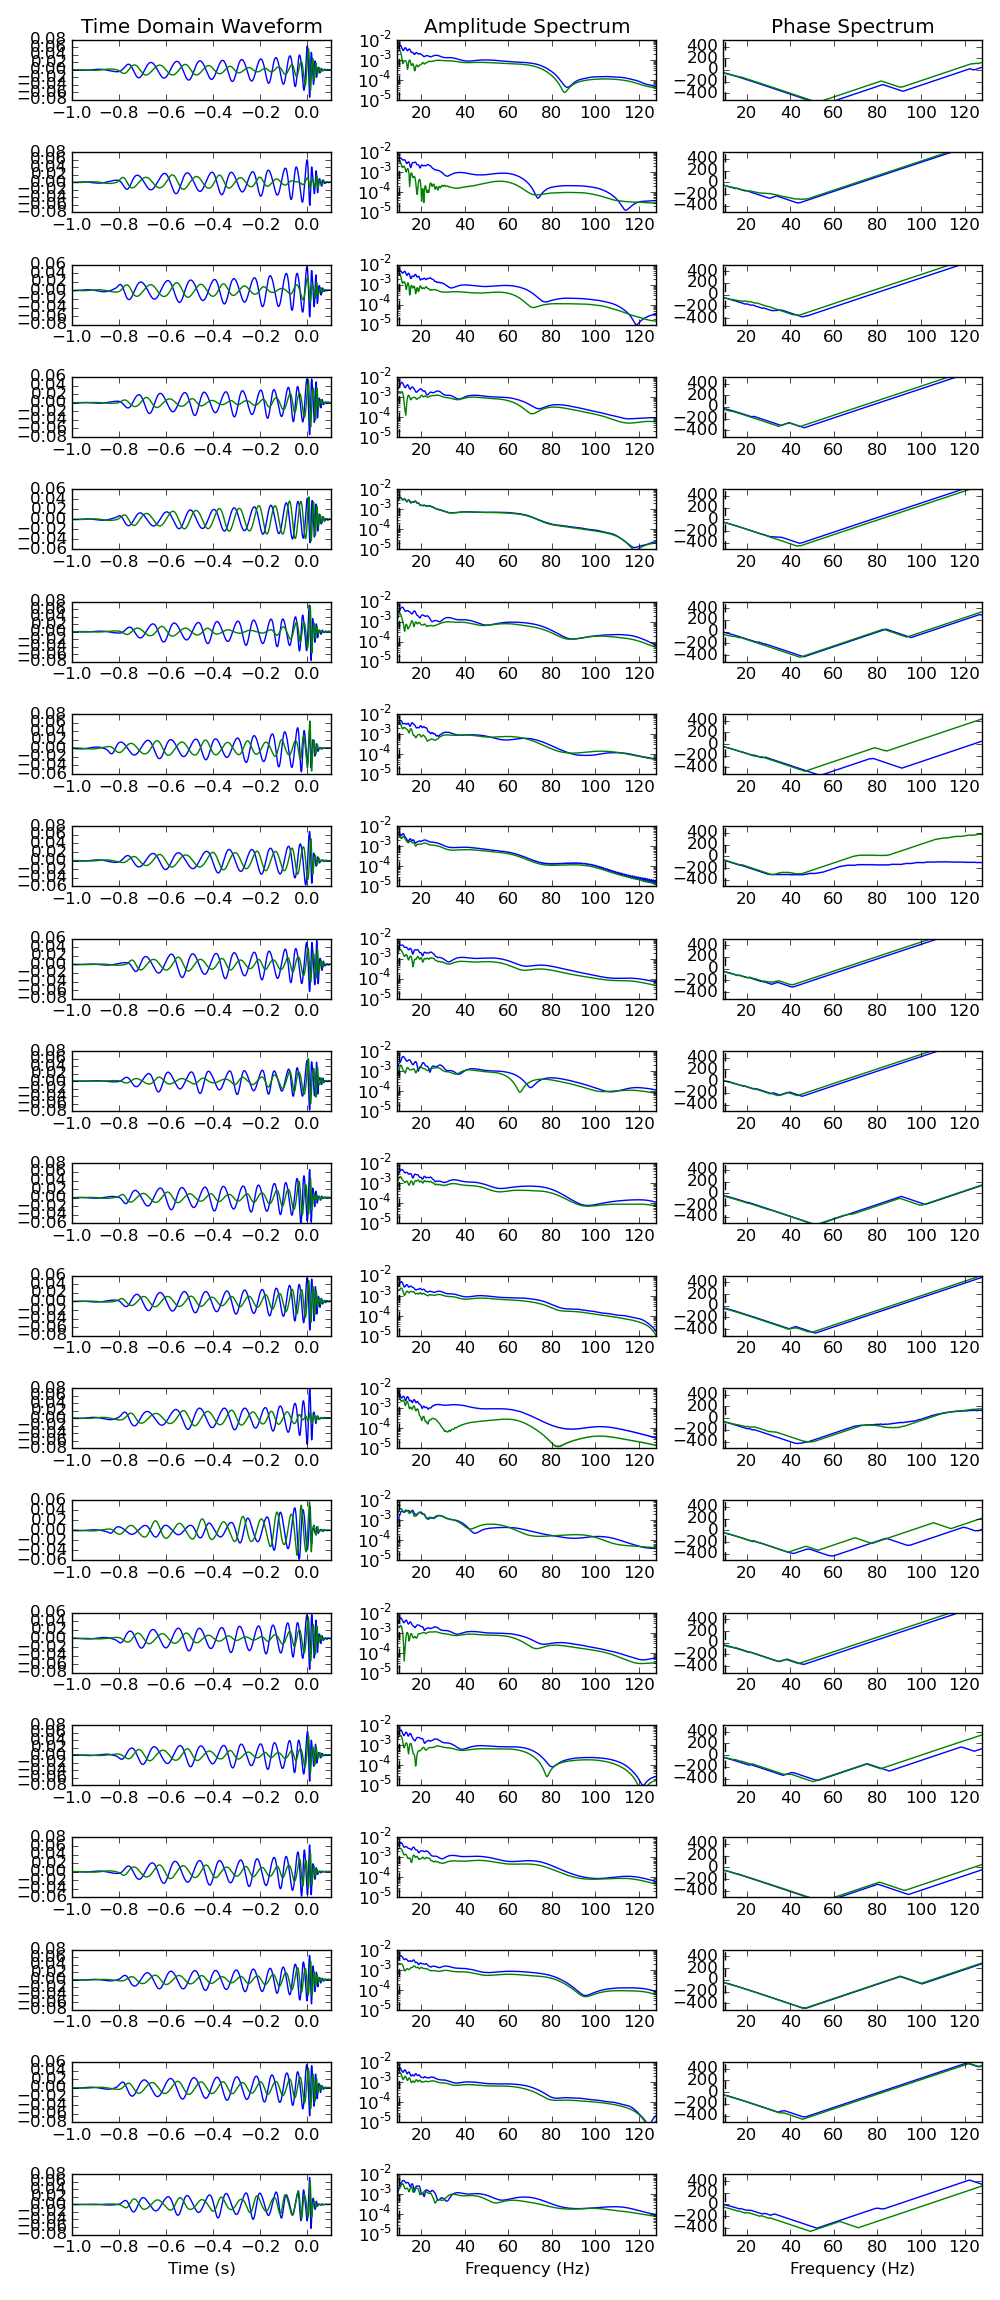
\includegraphics[width=0.4\textwidth]{figures/RO3-series_catalogue.png}
\caption{Waveforms that make up the RO3 catalog}
\label{fig:RO3_catalog}
\end{figure}

\end{document}
%
% ****** End of file bhextractor_paper.tex ******